\documentclass[12pt,a4paper]{report}
\usepackage{geometry}
\usepackage{hyperref}
\hypersetup{
  colorlinks=true,
  linkcolor=black,
  citecolor=black,
  filecolor=black,
  urlcolor=black
}
\usepackage{graphicx}
\usepackage{booktabs}
\usepackage{longtable}
\usepackage{array}
\usepackage{caption}
\usepackage{float}
\usepackage{amsmath}
\usepackage{cite}
\usepackage{setspace}
\usepackage{fontspec}
\usepackage{etoolbox}
\usepackage{titlesec}

\geometry{margin=1in}

% Set main font to Trebuchet MS - requires XeLaTeX or LuaLaTeX
\setmainfont{Trebuchet MS}

% Set 1.5 line spacing
\onehalfspacing

% Rename contents title
\renewcommand{\contentsname}{Table of Contents}

% Ensure chapters are displayed correctly with proper spacing
\titleformat{\chapter}[display]
  {\normalfont\huge\bfseries}{}{0pt}{\centering} % Ensures the title is centered and formatted properly
\titlespacing{\chapter}{0pt}{-40pt}{10pt} % Reduce space before & after the title

% Force override LaTeX default chapter spacing
\makeatletter
\patchcmd{\@makechapterhead}{\vspace*{50\p@}}{\vspace*{0pt}}{}{}
\patchcmd{\@makeschapterhead}{\vspace*{50\p@}}{\vspace*{0pt}}{}{}
\makeatother

% Adjusting spacing for sections
\titlespacing\section{0pt}{5pt}{5pt}

\begin{document}

% Custom title page as per user feedback
\begin{titlepage}
    \centering
    
\includegraphics[width=0.9\textwidth]{img/UCU.png}\\
    \vspace*{2cm}
    {\Huge\bfseries AgriBot: A Smart Irrigation, Soil Monitoring, and Pest Detection Robot for Ugandan Farms\par}
    \vspace{2cm}
    {\LARGE\itshape\textbf Project Proposal\par}
    \vspace{2cm}
    {\Large\textbf by:\par}
    \vspace{1cm}
    {\Large\textbf EZAMAMTI RONALD AUSTINE \par}
    \vspace{0.5cm}
    {\large S23B23-018\par}
    \vspace{0.5cm}
    {\large B24252\par}
    \vspace{1.5cm}
    {\large \today\par}
\end{titlepage}

\begin{center}
    {\LARGE\textbf Executive Summary}
\end{center}
\noindent
This project proposes the development of a multi-purpose robot system, "AgriBot"
to automate irrigation, soil monitoring, weed and pest detection
on Ugandan farms. AgriBot, with embedded systems and robotics, will
address critical agricultural inefficiencies. Agriculture is one of the pillars of the economy of Uganda, with nearly 68\% of its labor working in the sector and
making a contribution of approximately 24\% to the GDP. However, most of this sector relies on rain-fed agriculture,
making it highly vulnerable to climate change. AgriBot will utilize environmental
sensors, machine vision, thermal imaging, and Bluetooth‐based manual control for optimizing resource efficiency and mitigating these weaknesses. It will also possess a 5‐litre tank for storing pesticides to use for automatic spraying, especially on weeds and pests identified.
Future improvements aim to add poultry management features and AI decision-making capabilities.\\\\
\noindent
AgriBot is to be designed for use on any type of farm, but will first operate
with smallholder farmers, who make up approximately 80\% of Uganda's agricultural producers. This includes operators of greenhouses and nursery beds, many of whom are smallholders. Starting in controlled environments will allow refinement and safe pilot testing before scaling the solution to open spaces and large-scale farming operations.
The robot aligns with Uganda's NDP IV (2025/26 ‐ 2029/30) goals ~\cite{uganda2024ndpiv}, which emphasize agro‐industrialization, productivity improvement, and climate adaptation.
It is mapped to SDGs 2 (Zero Hunger), 9 (Industry, Innovation, and Infrastructure), and 13
(Climate Action)~\cite{colglazier2015sustainable}. The project will deliver an operational proof‐of‐concept prototype and a comprehensive plan for scalable deployment. 


% Set depth to include all sections and subsections in TOC
\setcounter{tocdepth}{3}

% Use tocloft package to customize TOC with dotted leaders
% \usepackage{tocloft}
% \renewcommand{\cftsecleader}{\cftdotfill{\cftdotsep}}

\tableofcontents
% \listoffigures
% \listoftables
\clearpage

\chapter{Chapter One: \\Introduction and Background}
Uganda's agriculture, while essential, faces numerous challenges. It remains largely rain-dependent and labor-based, making it susceptible to climate change, pests, and low productivity. The NDP IV (2025/26 - 2029/30) identifies agricultural productivity and mechanization as key to value addition and food security~\cite{uganda2024ndpiv}. However, the smallholder farmers, who constitute about 80\% of Uganda's agricultural landscape (owning farms with an average holding size of 1.3 hectares), face challenges such as inefficient irrigation, poor access to real-time soil data, and late detection of pests and weeds. These factors tend to contribute, low yields and hinder the sector's growth potential. For instance, Uganda's post-harvest losses are estimated at 40\% due to factors such as inadequate storage and pest infestations, further affecting food security.

\section{Problem Statement}
The majority of farmers in Uganda still rely on manual means for irrigation and pest control.  Less than 20\% apply modern farming methods. This non-adoption of mechanization results in significant water wastage (with some studies indicating losses of up to 60\% in traditional surface irrigation methods), late pest detection, and underutilization of farm potential. This situation is further compounded by limited access to affordable technology and infrastructure in rural areas, where only about 18\% of the rural population has access to electricity, a crucial input for many modern agricultural technologies. While large-scale farmers have begun to adopt mechanization, the gap remains widest among smallholder farmers, who contributed over 70\% of the country's food supply. An affordable and adaptable robotic solution could address these inefficiencies and empower farmers to improve their practices.

\section{Objectives}
\begin{itemize}
    \item To design and prototype a robotic system capable of soil moisture and temperature monitoring, automated irrigation, and detection of common weeds and pests in Ugandan crops.
    \item To integrate Bluetooth control for manual override, configuration, and data transmission, ensuring usability in areas with limited internet connectivity.\\
    \item To incorporate a 5-litre pesticide tank with a spraying mechanism triggered by weed and pest detection.
    \item To ensure the robot is modular and customizable based on farm size, garden layout, and farmer needs.
    \item To establish a roadmap for future features such as AI-based farming advice and poultry management support.
    \item To begin deployment in smallholder greenhouse and nursery bed environments for testing and refinement before scaling to all farm types.
\end{itemize}

\section{Justification}
AgriBot offers a scalable and affordable alternative to labor-intensive farming practices. The robot can optimize irrigation schedules, enabling farmers to use water more efficiently and reduce waste. Early detection of pests and weeds combined with targeted spraying reduces pesticide wastage and environmental impact. Temperature sensing ensures crops grow under optimal conditions. Customizability ensures the robot adapts to different farming scenarios. Future improvements could turn AgriBot into a multi-functional assistant capable of providing AI-based farming advice and supporting poultry health management. According to Uganda’s NDP IV~\cite{uganda2024ndpiv}, poultry is listed as a strategic commodity under the Agro-Industrialization Programme, which seeks to enhance productivity and resilience in livestock systems. By equipping AgriBot with sensors to monitor chick room temperatures, detect common poultry diseases and pests, and automate alerts for feed or water supply, the robot could help reduce mortality rates and economic losses in poultry production.\\
From an SDG perspective, integrating poultry management addresses goals such as:
\begin{itemize}
    \item \textbf{SDG 1 (No Poverty)}: Improves incomes of smallholder poultry farmers.
    \item \textbf{SDG 2 (Zero Hunger)}: Enhances food and nutrition security through improved protein supply.
    \item \textbf{SDG 3 (Good Health)}: Supports early detection of poultry diseases, reducing public health risks.
    \item \textbf{SDG 8 (Decent Work)}: Promotes sustainable employment in agriculture technology and livestock.
\end{itemize}

These enhancements will ensure AgriBot remains active throughout the year, \\minimizing human strain, and reinforcing national development goals related to inclusive agricultural transformation.

\chapter{Chapter Two: \\Literature Review}

\section{Current Developments in Precision Agriculture}
Recent academic literature strongly states the critical role of robotics and smart systems in modernizing agriculture. Albanese et al.~\cite{albanese2021automated} introduced a deep neural network system optimized for embedded pest detection. This work, published in the \textit{IEEE Journal on Emerging and Selected Topics in Circuits and Systems}, proves the feasibility of running machine learning models on low-power devices, an essential feature for AgriBot’s deployment in off-grid rural areas. The success of their model in detecting biotic stress supports the integration of edge‐AI in pest control. Specifically, their approach leverages a deep neural network architecture optimized for embedded systems, achieving high accuracy in pest detection while maintaining low computational overhead. This enables real-time monitoring and decision-making directly on the device, reducing the need for constant connectivity or cloud processing.

A study by Nomugisha and Dr Mwebaze~\cite{godwin2025smart} proposed a climate-resilient smart IoT framework tailored for smallholder maize farming in Uganda. This work directly relates to AgriBot’s context, highlighting the need for cost-effective IoT deployment, farmer feedback loops, and sensor-based decision-making to improve resilience against climate variability. Their framework integrates environmental sensors with data analytics to provide actionable insights to farmers, although it remains conceptual without a physical hardware prototype. AgriBot builds upon this by implementing a tangible robotic system that uses these principles in a field-deployable platform.

Wanyama et al.~\cite{wanyama2024systematic} performed a systematic review of Fourth Industrial Revolution (4IR) technologies in Sub-Saharan Africa, identifying critical gaps in the adoption of smart irrigation solutions. While their study confirms the transformative potential of AI and IoT in precision irrigation, it emphasizes the challenges faced by smallholder farmers—namely lack of affordability, infrastructure, and localized design. The review highlights the importance of modular, scalable, and locally adaptable technologies to overcome these barriers. AgriBot directly tackles these constraints through modular, locally sourced hardware and offline Bluetooth communication, making it accessible and practical for smallholder farmers.\\ \\ \\

Geetha Lekshmy et al.~\cite{geetha2022adaptive} proposed an adaptive IoT model that combines irrigation and pest control in a self-healing sensor network. While the system is innovative in handling sensor failures, it was primarily tested in controlled conditions and lacks practical deployment in African farm environments.
Their model uses redundancy and adaptive algorithms to maintain network reliability, which is critical for continuous monitoring. AgriBot bridges this gap by designing a field-deployable solution with direct input from Ugandan farmers, ensuring robustness and usability in real-world conditions.
\section{Identified Gaps in Research}
Despite strong academic evidence supporting the use of automation in agriculture, gaps remain in: (1) integration of pest detection with targeted spraying, (2) modular adaptability for different farm sizes, and (3) combining crop and poultry support systems into one platform. AgriBot’s design responds to these research and practice gaps, offering a solution that is both innovative and grounded in real-world agricultural needs.

Additional studies have explored the integration of machine learning and IoT in agriculture. For instance, recent advances in TinyML have enabled the deployment of lightweight neural networks on microcontrollers, facilitating real-time pest and disease detection in resource-constrained environments. These developments align with AgriBot’s goal of providing edge-based intelligence for timely interventions.

Furthermore, research into sensor fusion techniques has demonstrated improved accuracy in soil moisture and temperature monitoring by combining data from multiple sensor types. This approach enhances decision-making for precision irrigation, reducing water waste and improving crop health.

Studies on user-centered design in agricultural technology emphasize the importance of involving smallholder farmers in the development process to ensure usability and adoption. AgriBot’s iterative design and testing in greenhouse and nursery environments will reflect this principle, aiming to tailor the system to local needs and constraints.

Overall, the literature supports the potential of integrated robotic systems like AgriBot to transform smallholder agriculture in Uganda by addressing key challenges related to resource efficiency, pest management, and climate resilience.

\chapter{Chapter Three: \\Methodology}
\section{Methodology of the Proposed System}
The development of AgriBot will follow a systematic approach involving consultation with technical staff to acquire well-detailed system requirements. This will ensure the design aligns with practical needs and leverages expert insights. \\The methodology includes hardware design, software implementation, and rigorous testing and evaluation phases.

\section{Hardware Design}
\begin{itemize}
    \item Soil and Environmental Monitoring: Moisture, temperature, and pH sensors
    \item Precision Irrigation: Solenoid valve and pump with micro-sprinklers
    \item Pest and Weed Detection: ESP32-CAM or PiCamera
    \item Thermal Imaging: MLX90640 thermal sensor for plant monitoring
    \item Spraying Mechanism: 5-litre pesticide tank with actuated nozzle
    \item Chassis: Terrain-capable wheels and frame
    \item Power: Solar with battery backup
    \item Communication: Bluetooth (e.g, HC-05)
\end{itemize}

\section{Software Implementation}
\begin{itemize}
    \item Microcontroller Firmware (ESP32/Arduino)
    \item Machine Learning (TinyML for pest/weed recognition and heat stress)
    \item User Interface: Bluetooth mobile app for control and monitoring
\end{itemize}

\section{Testing and Evaluation}
\begin{itemize}
    \item Greenhouse and nursery testing
    \item Performance metrics: accuracy, water/pesticide use, usability, ROI
\end{itemize}

\section{Budget (UGX)}
\begin{tabular}{lr}
\toprule
Sensors (moisture, pH, temperature) & 800,000 \\
Camera and ML processing unit & 1,500,000 \\
Thermal sensor (MLX90640) & 450,000 \\
Motors, chassis, wheels & 800,000 \\
Spraying system (tank, nozzles, pump) & 700,000 \\
Bluetooth module and controller board & 500,000 \\
Solar and battery unit & 1,200,000 \\
Contingency Fund (Price fluctuations, unforeseen situations) & 550,000 \\
\midrule
\textbf{Total} & \textbf{8,000,000 UGX} \\
\bottomrule
\end{tabular}
\vspace{2cm}
\section{Workplan (Four Weeks)}
\begin{spacing}{1.5}
\begin{table}[H]
\centering
\renewcommand{\arraystretch}{1.5}
\begin{tabular}{|c|l|}
\hline
\textbf{Day} & \textbf{Activity} \\
\hline
1-2 & Team formation and briefing (5-7 members) \\
\hline
3-4 & Stakeholder consultation and user needs analysis \\
\hline
5-7 & Procurement of components (sensors, motors, thermal camera) \\
\hline
8-11 & Hardware assembly (chassis, sensors, sprayer integration) \\
\hline
12-15 & Firmware programming and mobile interface development \\
\hline
16-19 & Machine learning model training and integration \\
\hline
20-23 & Field testing in greenhouse/nursery environments \\
\hline
24-26 & Data collection and performance analysis \\
\hline
27-28 & Final report writing and prototype demonstration \\
\hline
\end{tabular}
\caption{Workplan for AgriBot Project}
\end{table}
\end{spacing}

\renewcommand{\bibname}{References}
\addcontentsline{toc}{chapter}{References}
\bibliographystyle{IEEEtran}
\bibliography{AgriBot_References}

\appendix
\chapter*{Appendix:}
\addcontentsline{toc}{chapter}{Appendix}

\begin{figure}[H]
    \centering
    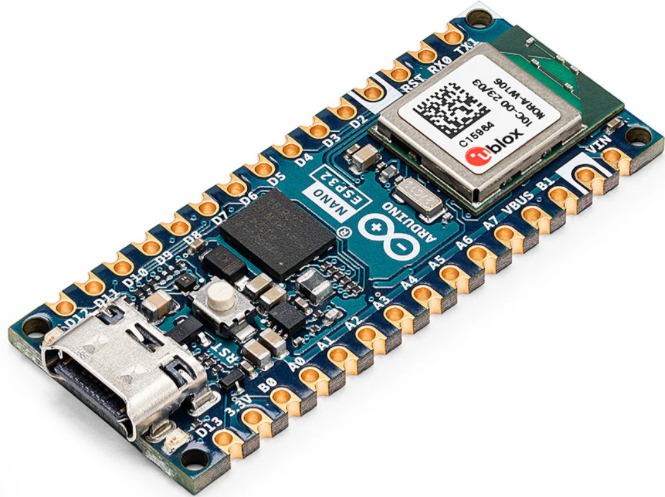
\includegraphics[width=0.8\textwidth]{img/Arduino Nano Esp32 (Original).png}
    \caption{Arduino Nano Esp32 Source: [https://store.arduino.cc/products/nano-esp32]}
\end{figure}

\begin{figure}[H]
    \centering
    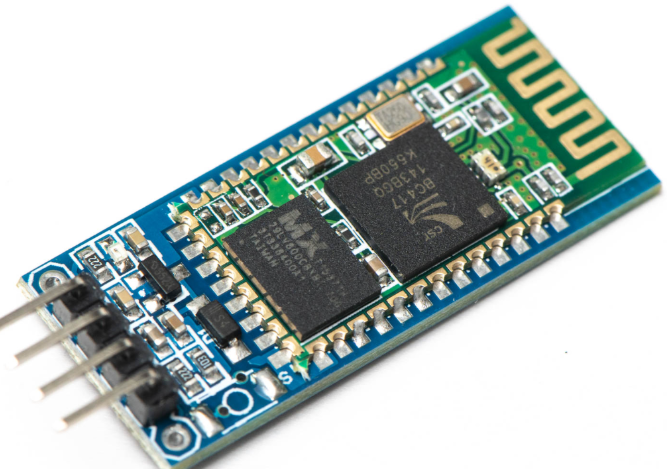
\includegraphics[width=0.8\textwidth]{img/HC05-HC06 Bluetooth Module.png}
    \caption{HC05/6 Bluetooth Module Source:[https://images.app.goo.gl/WEQmqYtAf1ApzWFW7]}
\end{figure}

\end{document}
